Docker es una plataforma abierta diseñada para el desarrollo, despliegue y ejecución
de aplicaciones \cite{DockerOverview2021}. La idea fundamental que reside detrás de
Docker es la de separar la infraestructura de las aplicaciones de manera que se pueda
entregar el \textit{software} rápidamente.

Por debajo, Docker ofrece una plataforma que otorga la habilidad de empaquetar y
ejecutar las aplicaciones en un entorno aislado llamado ``contenedor'' (\textit{container}).
Entre otras características, un contenedor permite ejecutar una aplicación de forma
segura sobre el host en cuestión. La pregunta que surge es, ¿qué es un contenedor?

\subsubsection*{Contenedores}
Un contenedor es una unidad estándar \textit{software} que empaqueta código y todas
sus dependencias de manera que la aplicación se ejecuta rápidamente y de forma fiable
bajo múltiples entornos de ejecución \cite{WhatContainerApp}. Una imagen Docker
es un paquete ligero, independiente y ejecutable que incluye absolutamente todo
lo necesario para poder ejecutar una aplicación: desde el código en sí hasta el
\textit{runtime}, herramientas del sistema, librerías y configuraciones.

Durante la ejecución, una imagen se convierte en un contenedor que se ejecuta sobre
la máquina Docker (\textit{Docker Engine}), la cual se encuentra disponible en 
entornos Linux y Windows.

Al fin y al cabo, los contenedores nos aseguran que una aplicación que hemos 
desarrollado se va a ejecutar de la misma manera en una máquina u otra. El uso del
motor Docker permite ejecutar múltiples contenedores sobre un mismo anfitrión
sin añadir demasiada carga en el sistema e indiferentemente de la infraestructura
que exista por debajo (figura \ref{fig:docker-containers-rt}):

\begin{figure}[H]
    \centering
    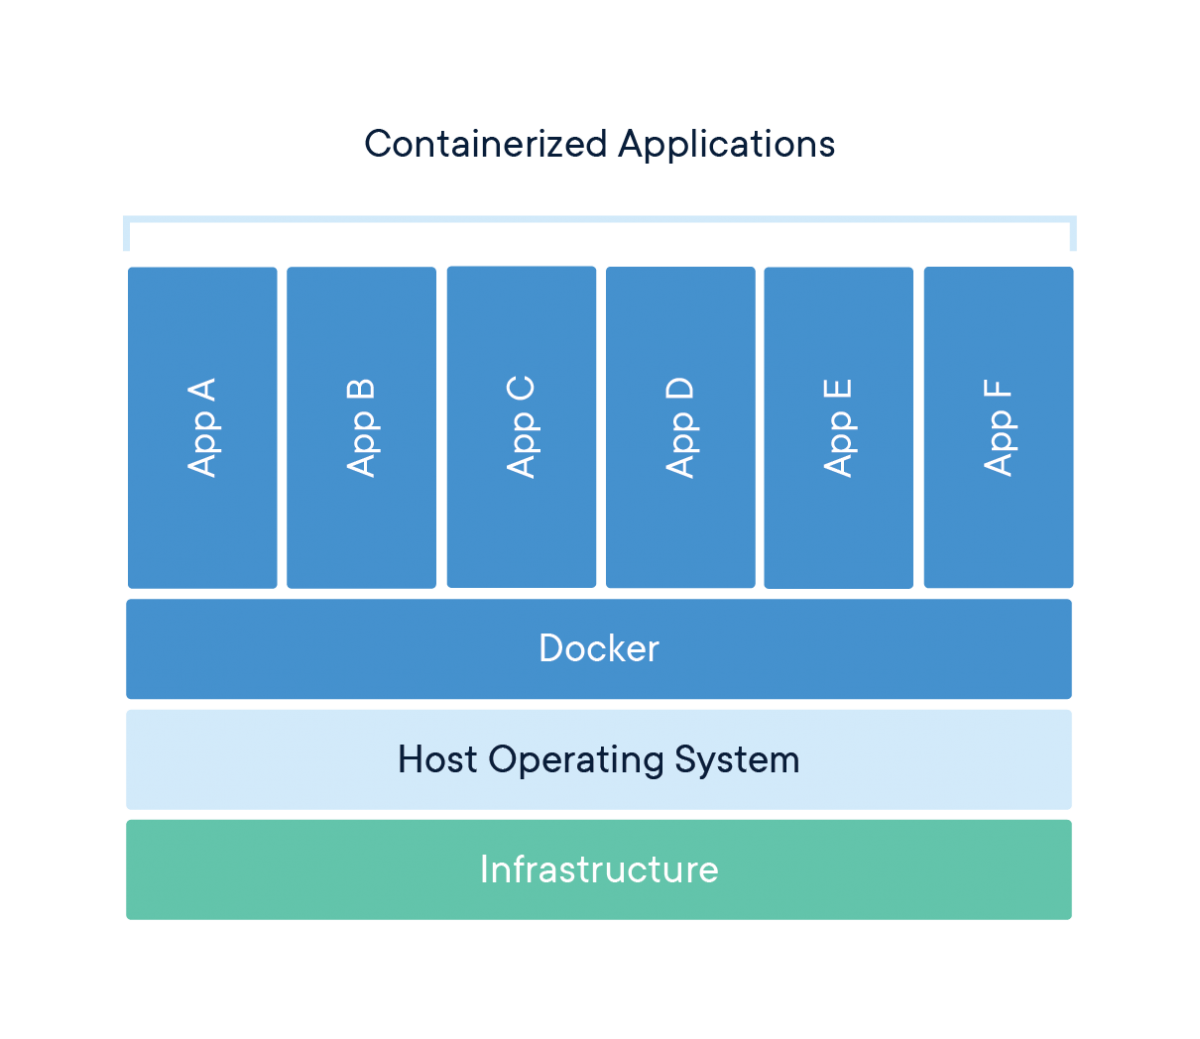
\includegraphics[width=.7\linewidth]{pictures/container-what-is-container.png}
    \caption{Distribución de los contenedores sobre el motor de ejecución de Docker \cite{WhatContainerApp}.}
    \label{fig:docker-containers-rt}
\end{figure}

La distribución de los contenedores mostrada en la figura \ref{fig:docker-containers-rt}
puede parecerse mucho a la distribución que tendríamos en una máquina virtual. Sin embargo,
hay varias características que lo distinguen principalmente:

\begin{enumerate}
    \item Un contenedor se ejecuta directamente sobre la máquina anfitriona, mientras
          que una máquina virtual requiere de un hipervisor.
    \item Un contenedor es una abstracción de la capa de aplicación que encapsula
          el código y las dependencias juntas, mientras que una máquina virtual es
          una abstracción de una capa física \textit{hardware}.
    \item Un contenedor comparte el kernel con el sistema operativo anfitrión, por lo
          que tiene un gran rendimiento; mientras, una máquina virtual ejecutará su
          propio kernel sobre el hipervisor del sistema operativo anfitrión.
    \item El espacio que necesita un contenedor es muy pequeño en comparación con el
          de una máquina virtual, que engloba y encapsula un sistema operativo al
          completo.
\end{enumerate}

\begin{figure}[H]
    \centering
    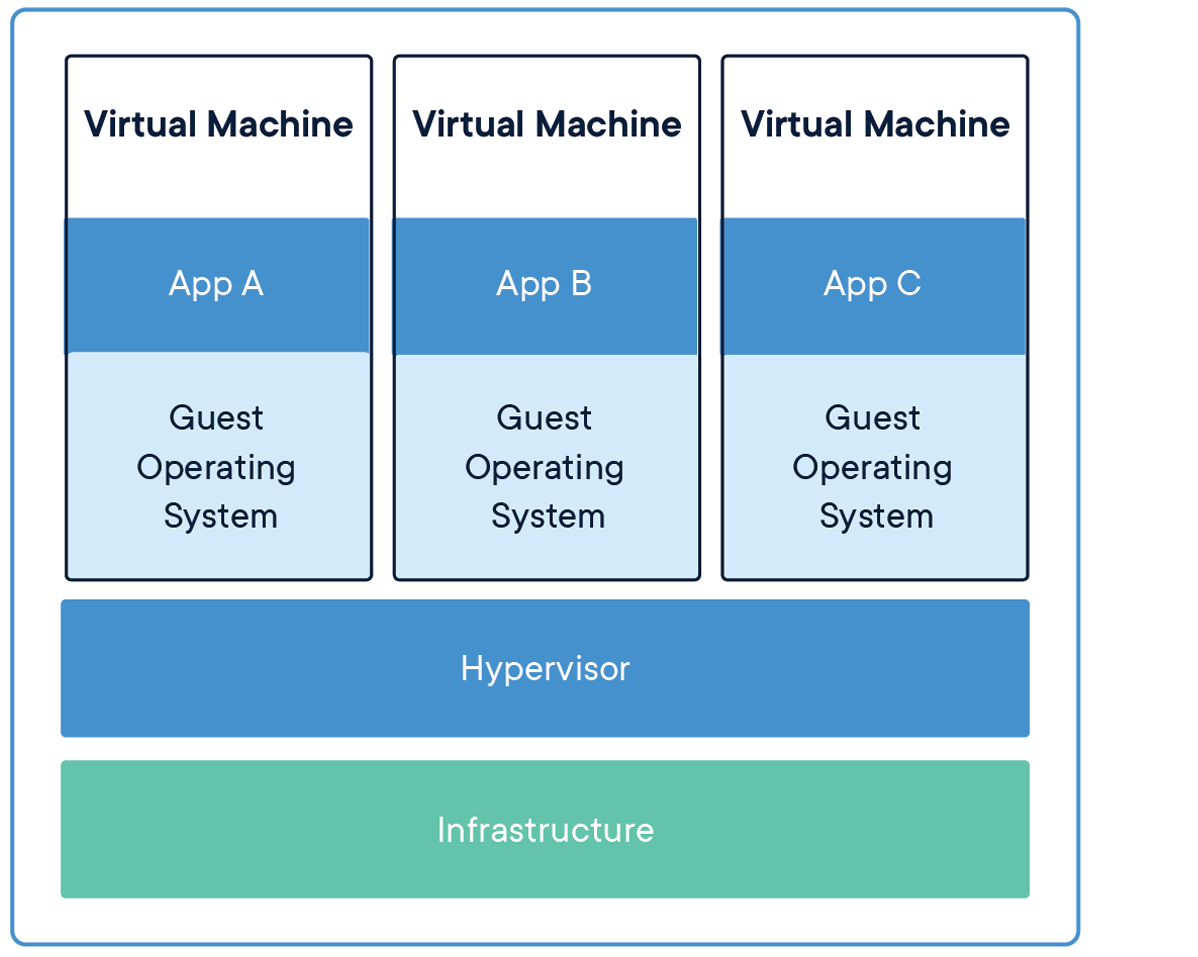
\includegraphics[width=.7\linewidth]{pictures/container-vm-whatcontainer_2.png}
    \caption{Capas de abstracción de una máquina virtual sobre una máquina anfitriona \cite{WhatContainerApp}.}
    \label{fig:vm-layers}
\end{figure}

En la figura \ref{fig:vm-layers} se puede apreciar cómo una máquina virtual añade
muchas más capas de abstracción que ralentizan el rendimiento. Sin embargo, esto
no quiere decir que sean una mala alternativa: la realidad es que se combinan las
dos para obtener una gran flexibilidad para desplegar aplicaciones -- contenedores
cuando se quiere ejecutar algo directamente sobre el anfitrión; máquinas virtuales
para emular \textit{hardware} y que ejecuten en su interior contenedores para ejecutar
aplicaciones fácilmente.

La evolución y constante mantenimiento de los contenedores ha generado lo que se
conoce como estándar de la industria ``\textit{containerd}''. Este estándar define
claramente qué arquitectura debe tener un contenedor por debajo y está en constante
evolución a medida que la industria crece y madura.

Además, la especificación anterior ha pasado de ser un mero estándar a una aplicación
en sí de gestión y orquestación de contenedores, permitiendo que aplicaciones distintas
de Docker hagan uso de la arquitectura basada en contenedores aprovechando la OCI:
\textit{Open Container Initiative}

\begin{figure}[H]
    \centering
    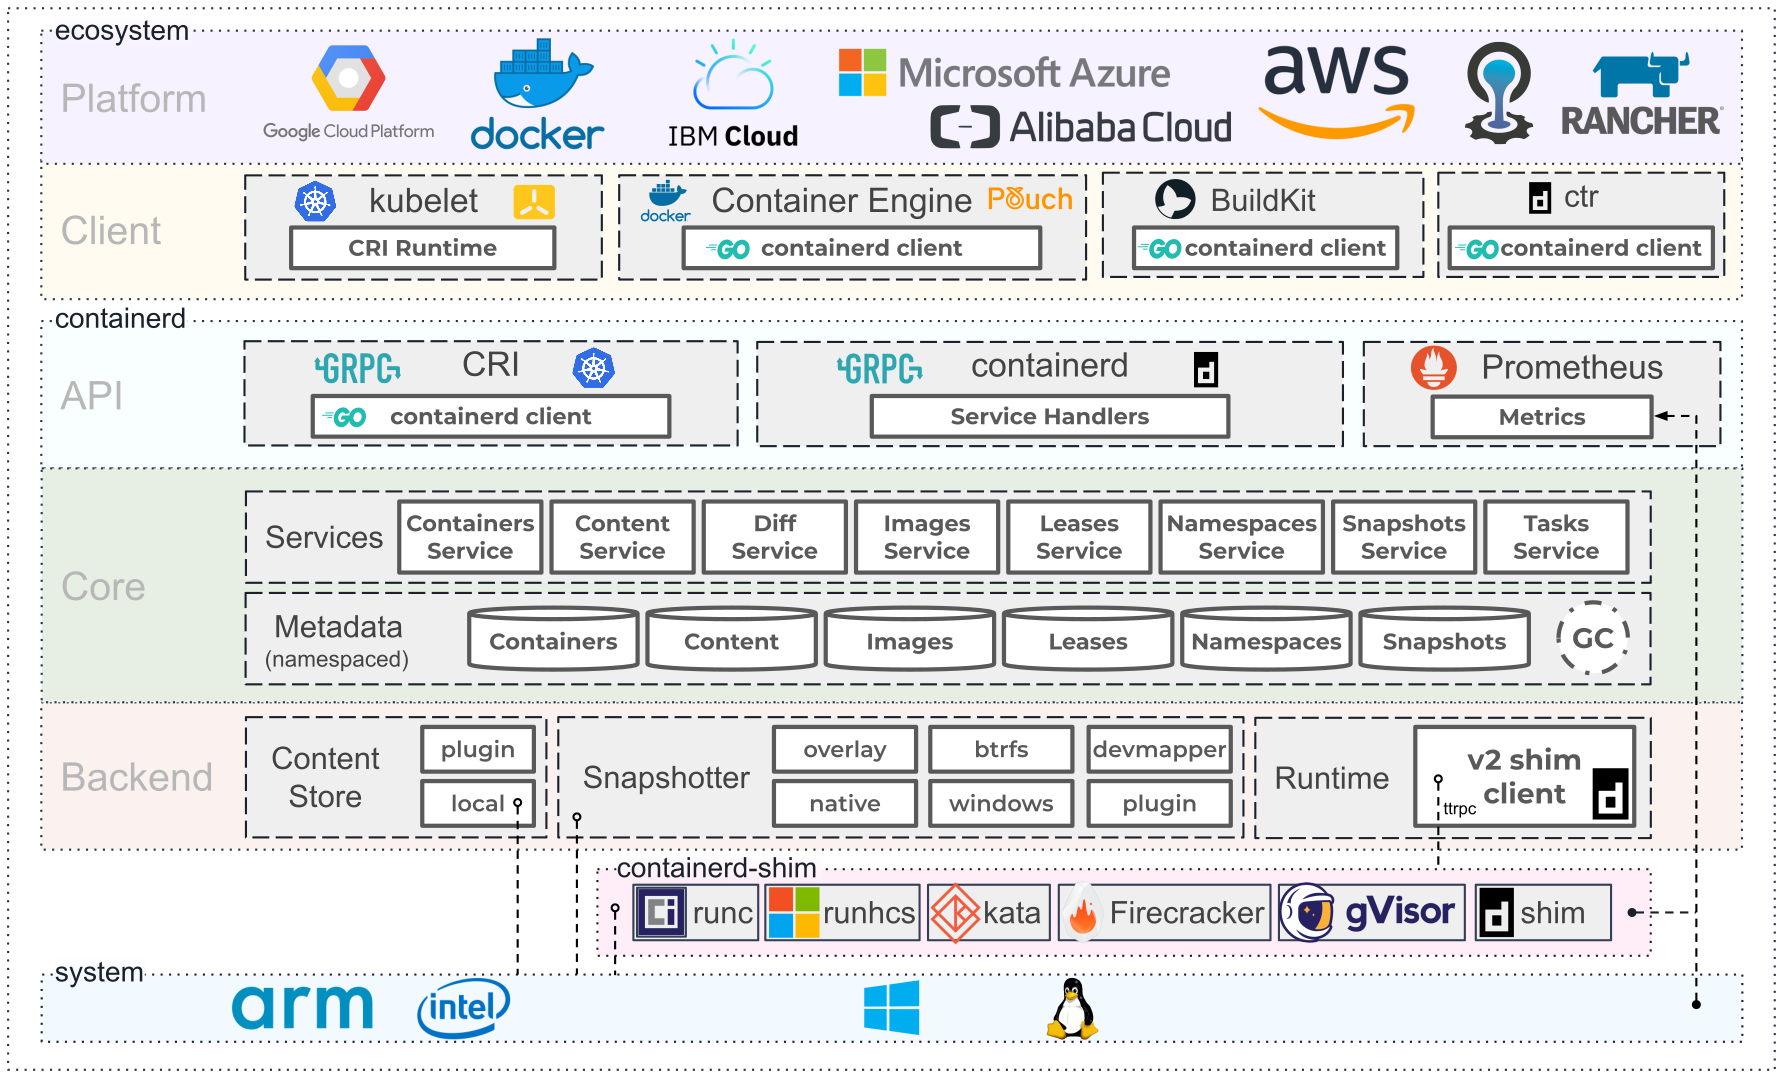
\includegraphics[width=.7\linewidth]{pictures/containerd-arch.png}
    \caption{Entorno de ejecución de \textit{containerd} basado en \texttt{runC} de la OCI \cite{Containerd}.}
    \label{fig:containerd-arch}
\end{figure}

\subsubsection*{Docker Engine}
El motor de ejecución de Docker establece la arquitectura de ejecución \textit{de facto}
que es utilizable desde distintas distribuciones Linux y servidores Windows \cite{ContainerRuntimeDocker}.

\begin{figure}[H]
    \centering
    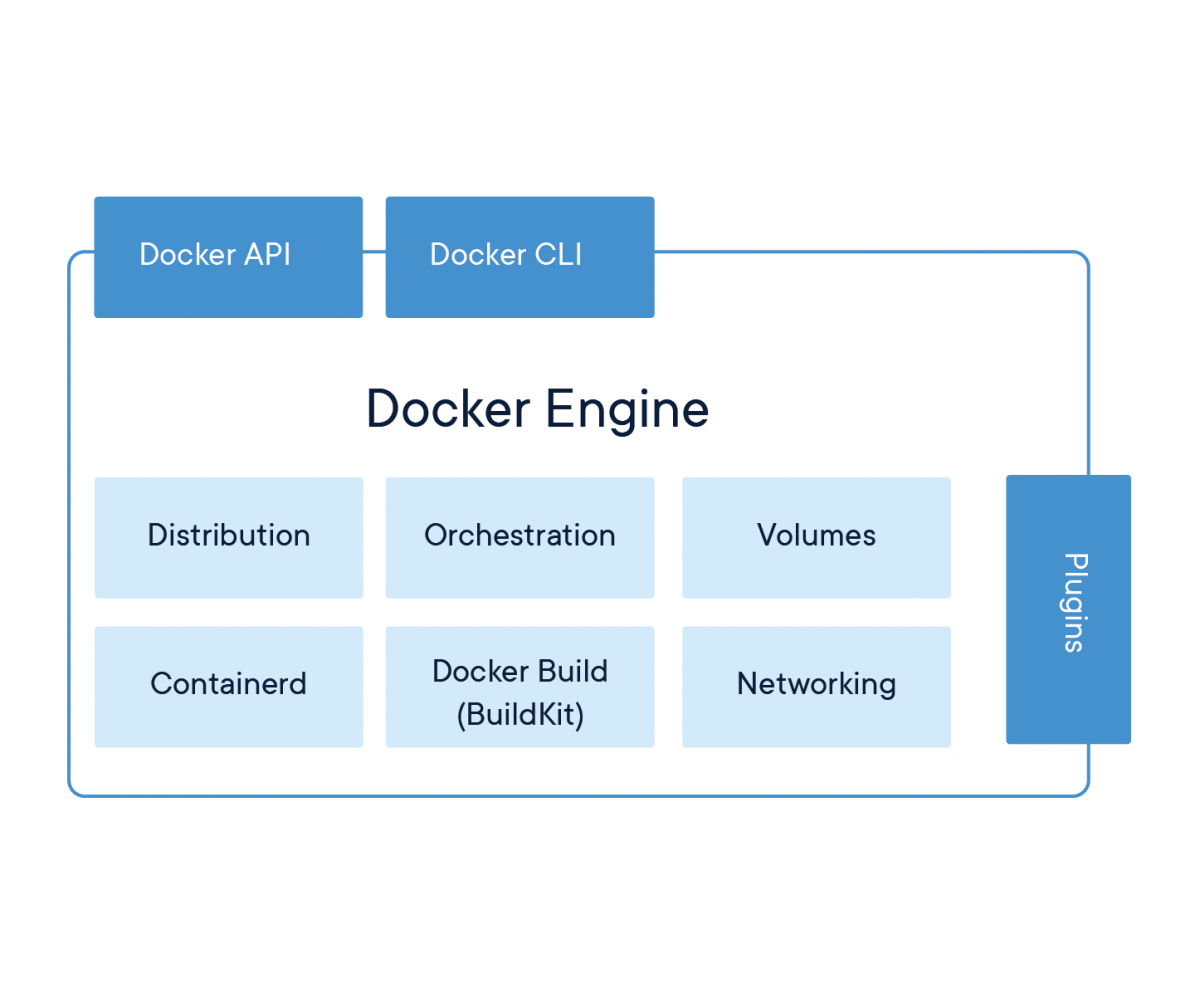
\includegraphics[width=.7\linewidth]{pictures/docker-engine.png}
    \caption{Arquitectura del entorno de ejecución de Docker \cite{ContainerRuntimeDocker}.}
    \label{fig:docker-engine}
\end{figure}

El motor de ejecución de Docker se compone de una gran cantidad de elementos que
encapsulan de forma uniforme multitud de aptitudes de un sistema operativo o una
aplicación (figura \ref{fig:docker-engine}). Este entorno de ejecución sin embargo
es complejo ya que engloba multitud de elementos físicos, como pueden ser las interfaces
de red y los volúmenes.

Esto resulta fundamental ya que los contenedores Docker no tienen ni que confiar en
la red del anfitrión: tienen su propio \textit{stack} de red para realizar las comunicaciones
que necesiten. Con el motor de ejecución de Docker se busca solventar esos problemas
``\textit{dependency hell}'' que se han comentado anteriormente y la situación de ``en mi equipo
funciona''.

De los elementos mostrados en la figura \ref{fig:docker-engine}, se tiene que son:

\begin{itemize}
    \item \textit{Distribution}: la distribución Linux en la que se basa el contenedor.
          Actualmente, Docker solo permite ejecutar contenedores basados en Linux.
    \item \textit{Orchestration}: cuando hay múltiples contenedores, la orquestación
          es el proceso por el cual el motor de ejecución de Docker gestiona y
          maneja qué contenedores se ejecutan, cómo se comunican, cuáles hay que
          crear nuevos y cuáles eliminar. Es de las partes más complejas que existen
          en el mundo de los contenedores y ha evolucionado a clústers mucho más
          completos (y complejos) como Kubernetes o Docker Swarm.
    \item \textit{Volumes}: los volúmenes (conjuntos de datos) que se manejan en los
          contenedores. Debido a su arquitectura cerrada, los datos que genera un
          contenedor solo están visibles para ese contenedor mientras este esté en
          ejecución. Cuando finalice, todos los datos no persistentes son eliminados.
    \item \textit{Containerd}: el estándar y cliente de ejecución y manejo de los
          contenedores a muy bajo nivel.
    \item \textit{Docker Build (BuildKit)}: herramienta de libre distribución que
          transforma los ficheros \texttt{Dockerfile} en imágenes Docker, listas
          para ser usadas y distribuídas.
    \item \textit{Networking}: \textit{stack} de red completo que se pone a disposición
          de cada contenedor Docker. Cada aplicación puede crear su propio dispositivo
          de red que cumpla con los requisitos que necesita. Existen varios tipos de
          adaptadores: \textit{bridge}, \textit{NAT} y \textit{host}. El primero
          se emplea para realizar comunicaciones a través de red entre distintos
          contenedores; el segundo para realizar comunicaciones con el exterior
          mediante una conexión de red completamente independiente a la del anfitrión;
          la tercera para compartir la interfaz de red del anfitrión con el contenedor,
          como si fuese una aplicación interna.
\end{itemize}

Con todo lo anterior, una aplicación puede ejecutarse muy fácilmente en cualquier
equipo que integre el motor de ejecución de Docker.

